\chapter{Implementace}
Pro implementaci programu převádějícího OSM data do formátu vyhledávacího grafu
jsme zvolili v~první části Python, protože pro něj existuje široké množství
knihoven, které nám pomohly při řešení jednotlivých dílčích problémů. Při
vytváření spojek mezi cestami a jejich následné kontrole již ale nedostačoval,
proto jsme tuto a další části implementovali v~jazyce C. Mezi těmito částmi
předáváme data pomocí Protocol Bufferu v~souboru. Vyhledávání je také
implementováno v~jazyce C kvůli rychlosti a paměťové nenáročnosti.

\section{Použité knihovny a pomocné programy}
Během implementace programu pro přípravu dat jsme se snažili použít co nejvíce
již existujících knihoven a programů pro jednotlivé řešené problémy. Všechny
tyto knihovny a programy jsou nutné pro spuštění a používání našeho programu. 

\medskip
\noindent Používáme tyto pomocné programy, údaj v~závorce udává licenci:
\begin{itemize}
	\item Výřez s~městem z~dat pro republiku vyrábíme pomocí {\tuc
	Osmconvert} (GNU AGPL).\\
	\url{http://wiki.openstreetmap.org/wiki/Osmconvert}
	\item Pro práci s~Protocol Buffery v~Pythonu využíváme třídy generované
	kompilátorem {\tuc protoc} (BSD New).\\
	\url{http://code.google.com/p/protobuf/}
	\item Pro práci s~Protocol Buffery v~C využíváme funkce a struktury
	generované kompilátorem {\tuc protobuf-c} (BSD 2-Clause).\\
	\url{https://github.com/protobuf-c/protobuf-c}
\end{itemize}

\noindent V~programech napsaných v~Pythonu využíváme následující knihovny:
\begin{itemize}
	\item Na parsování konfiguračních souborů používáme {\tuc PyYAML}
	(MIT).\\
	\url{http://pyyaml.org/wiki/PyYAML}
	\item Na parsování OSM XML používáme {\tuc imposm.parser} (Apache).\\
	\url{http://imposm.org/docs/imposm.parser/latest/}
	\item Souřadnice konvertujeme pomocí {\tuc pyproj} (MIT).\\
	\url{http://code.google.com/p/pyproj/}
	\item Pro hledání komponent grafu využíváme {\tuc networkx} (BSD).\\
	\url{http://networkx.github.io/}
\end{itemize}

\noindent V~programech napsaných v~C využíváme následující knihovny:
\begin{itemize}
	\item Datové struktury, dynamická pole a další funkce zajišťuje
	{\tuc LibUCW} (GNU LGPL).\\
	\url{http://www.ucw.cz/libucw/}
	\item Výpočty se zeměpisnými souřadnicemi provádí {\tuc PROJ.4} (MIT).\\
	\url{http://trac.osgeo.org/proj/}
\end{itemize}

Program osmconvert je již zahrnut ve zdrojovém kódu, ostatní knihovny je
potřeba nainstalovat zvlášť.

\section{Datové struktury}
V~průběhu celé přípravy vyhledávacích dat často využíváme několik struktur,
které nyní popíšeme. Datové struktury využívané jen v~konkrétních případech
popíšeme u~těchto případů.

Při přípravě dat používáme několik {\tuc hešovacích tabulek}. Často potřebujeme
získat uzel respektive cestu s~konkrétním identifikátorem, pro tento účel nám
slouží tabulky \verb|nodesIdx| respektive \verb|waysIdx|. V~Pythonu jsou
reprezentovány typem slovník, v~C využíváme součást knihovny LibUCW
\verb|hashtable|. V~obou případech je klíčem OSM identifikátor objektu a
hodnotou index do pole uzlů resp. cest, kde je daný objekt uložen.

U~každé cesty je v~datech uložen seznam uzlů, přes které prochází. Je ale vhodné
mít i pro každý uzel uložen seznam cest, na nichž leží. Pro tento účel
máme seznam \verb|nodeWays|. Je to seznam seznamů, kdy pod indexem $i$ je seznam
všech identifikátorů cest, které prochází uzlem na pozici $i$ v~poli všech uzlů.
V~Pythonu jde o~seznam seznamů, v~C je to rostoucí pole rostoucích polí
z~LibUCW.

Během zpracování hledáme uzly blízké daným uzlům. Abychom pro každé takové
hledání nemuseli procházet všechny uzly, vytvoříme si na začátku {\tuc mřížku}.
Tato mřížka dělí plochu mapy na čtverce $20 \times 20$\,m a v~každém čtverci si
uložíme seznam identifikátorů vrcholů, které v~něm leží. Poté nám při hledání
sousedů bodu stačí zjistit, do kterého čtverce patří, a následně prohledat jen
několik okolních čtverců.

Mřížka je vhodnou strukturou pro rozdělení plochy, protože zástavba ve městě je
poměrně homogenní, tudíž zde nejsou příliš velké volné plochy, kde bychom
zbytečně plýtvali pamětí, ani místa, kde by počet bodů ve čtverci mřížky byl
obtížný na zpracování.

V~Pythonu se jedná o~třídu \verb|Raster|, která při vytvoření vyrobí mřížku
z~mapy. Mřížka je uložena v~atributu \verb|raster|, třída má metodu
\verb|getBox(x,y)|, která pro bod se souřadnicemi $(x,y)$ vrátí tuple se
souřadnicemi buňky, ve které se bod nachází. Mřížka \verb|raster| je seznam
seznamů seznamů.

V~C je mřížka reprezentována strukturou \verb|raster_t|. Samotná mřížka je prvek
\verb|raster| této struktury. V~souboru \verb|raster.h| jsou definovány funkce
pro práci s~mřížkou. Funkce \verb|makeRaster(map_t map)| vyrobí z~mapy mřížku a
vrátí ji. Funkce \verb|getRasterBox(raster_t raster, int64_t x, int64_t y)|
dostane jako paramter mřížku a souřadnice bodu a vrátí pole se dvěma prvky --
souřadnicemi buňky, kde se bod nachází. Mřížka \verb|raster| je reprezentována
polem polí rostoucích polí z~knihovny LibUCW.

\medskip


\section{Stažení dat OSM}
Abychom mohli připravovat data pro vyhledávání, musíme nejprve získat data OSM
pro dané město. O~tuto činnost se stará skript \verb|prepare.sh|, který stáhne
data pro celou Českou republiku a pomocí programu \verb|osmconvert| z~ní vyřízne
obdélník s~městem. Ten uloží jako \verb|praha.osm|\footnote{Program byl
připravován pro vyhledávání tras po Praze, proto soubory obvykle obsahují název
praha.} k~dalšímu zpracování.

\section{Příprava dat SRTM}
Kromě dat OSM potřebujeme i údaje o~výškách z~projektu SRTM. Protože tato data
se, narozdíl od dat OSM, nebudou aktualizovat, není pro jejich stažení skript,
ale je nutné do složky \verb|osm| nahrát soubory \verb|.hgt|, které pokrývají
obdélník s~městem. Pomocí programu \verb|merge-srtm| se \verb|hgt| soubory spojí
do jedné velké tabulky, která je uložena jako \verb|heights.txt|. Její první
řádek obsahuje rozsah pokrývaný SRTM tabulkou a další řádky pak obsahují tabulku
výšek.

\section{Klasifikace dat}
Před dalším zpracováním potřebujeme data OSM převést do formátu pro přípravu dat (premap).
K~tomuto účelu slouží program \verb|parse.py|, který si načte konfigurační soubory
a podle nich rozdělí jednotlivé uzly a cesty do kategorií. Současně také přidá
k~uzlům údaje o~nadmořské výšce a jejich souřadnice převede do UTM. Následně smaže 
všechny uzly, které neleží na žádné cestě, a uloží data do souboru ve formátu 
formátu premap.

Konfigurační soubory jsou soubory ve formátu YAML \cite{yamlspec}. Používají se následující
konfigurační soubory:
\begin{itemize}
	\item \verb|types.yaml| pro rozdělení cest a multipolygonů do
kategorií 
	\item \verb|area.yaml| pro určení, zda je daný objekt plochou
	\item \verb|tunnel.yaml| pro určení, zda je daný objekt tunelem,
	průchodem či jinou podobnou stavbou
	\item \verb|bridge.yaml| pro určení, zda je daný objekt mostem nebo na
	nějakém mostě leží
\end{itemize}

Konfigurační soubory mají následující formát:
\begin{verbatim}
BARRIER: 
    barrier : "*"
    waterway:
        - river
        - canal
WATER:
    waterway:
        - riverbank
        - stream
\end{verbatim}
Konfigurační soubor se skládá z~několika slovníků, u~každého klíč určuje, jaká
kategorie resp. hodnota se přiřadí. Hodnotou slovníku první úrovně jsou slovníky
druhé úrovně, které určují, za jakých podmínek se hodnota přiřadí. Přiřazuje se
vždy, když je splněna alespoň jedna podmínka. 

Ve slovnících druhé úrovně je klíčem vždy klíč vlastnosti objektu OSM. Hodnota může
být dvou druhů. Buď je to \verb|"*"|, pak stačí, že se shoduje klíč vlastnosti
OSM a na hodnoty se nehledí, nebo je hodnota slovníku seznam hodnot objektu OSM.
Pokud má objekt OSM pro daný klíč jednu z~těchto hodnot, je  podmínka splněna. 

V~příkladu rozdělujeme do kategorií \verb|BARRIER| a \verb|WATER|. Pokud má
objekt OSM nějaký atribut s~klíčem \verb|barrier|, je tomuto objektu přiřazena
kategorie \verb|BARRIER| nezávisle na hodnotě tohoto klíče. Obdobně je jako
\verb|BARRIER| označen objekt OSM, který má atribut s~klíčem \verb|waterway| a
hodnotou \verb|river|. Pokud má ale objekt atribut s~klíčem \verb|waterway| a
hodnotou \verb|stream|, je klasifikován jako \verb|WATER|.

Při procházení uzlů jim přiřazujeme ze SRTM výšku a převádíme jejich souřadnice
do UTM. Pomocí metody \verb|calcHeight| spočítáme nadmořskou výšku daného uzlu a
následně jeho souřadnice převedeme do UTM. Navíc {\tuc vynásobíme souřadnice UTM
desíti}, čímž bude jednotkou 10\,cm. Taková přesnost nám stačí a můžeme všechny
výpočty provádět v~celých číslech.

Následně vytvoříme hešovací tabulku \verb|nodeWays| a jejím průchodem zjistíme, které
uzly neleží na žádných cestách, a tyto uzly smažeme. Nakonec převedeme data do
formátu premap a uložíme jako soubor \verb|praha-pre.pbf| do složky \verb|data|.

\section{Převod multipolygonů na cesty}
S~multipolygony se v~původní formě pracuje obtížně, protože se jejich obvod
skládá z~neseřazených cest. Pro naše účely se hodí vytvořit cesty reprezentující
obvod multipolygonu. Těchto cest může být více, protože multipolygon se může
skládat z~více komponent. 

Pro každý multipolygon si vytvoříme seznam všech vnějších cest. Pak vytvoříme
seznam sousedů \verb|neighs|, který pro každý uzel na některé z~vnějších cest
obsahuje jeho sousedy na těchto cestách. Ve správném případě by takto měl každý
uzel mít dva sousedy. Pokud tomu tak není, skončíme s~chybou. Poté vybereme
jeden uzel na obvodu a postupujeme po jeho sousedech, dokud se do něj opět
nevrátíme. Použité cesty smažeme ze seznamu všech cest a opakujeme, dokud nějaké
cesty zbývají. Pokud se vrátíme na vytvářenou cestu mimo první vrchol, skončíme
s~chybou.

\section{Spojení budov}
Při spojování bloků budov do jejich obrysu nejprve vytvoříme graf sousednosti
budov. Pro jeho reprezentaci použijeme knihovnu \verb|networkx|. Jednotlivé
budovy budou vrcholy v~grafu, pokud budovy sousední, bude mezi jejich vrcholy
hrana. Graf sousednosti vytváříme funkcí \verb|makeNeighGraph|.

Do grafu nejprve přidáme všechny budovy jako vrcholy. Následně procházíme
všechny uzly a u~každého zkoumáme cesty, které jím prochází. Pokud jde jen
o~budovy, pak mezi první budovou a všemi ostatními vytvoříme v~grafu hrany. Pokud
mezi cestami je i nějaká, která není budovou, pak jsou všechny sousední budovy
označeny za vadné a hrany nepřidáváme.

Když máme graf vytvořen, procházíme ve funkci \verb|mergeComponents| jednotlivé
jeho komponenty a ze všech cest v~komponentě, které nejsou vadné, se pokoušíme
vytvořit cestu. Pokud se to povede, přidáme ji mezi cesty a původní cesty
jednotlivých budov vložíme do seznamu ke smazání. Nakonec funkcí
\verb|removeMerged| smažeme všechny budovy, které jsme nahradili jejich obvodem.

Když vytváříme cestu z~obvodu bloku budov pomocí funkce \verb|mergeWays|,
postupujeme obdobně jako při převodu multipolygonů na cesty. Vytvoříme si seznam
\verb|neighs|, který obsahuje pro každý bod na některé ze spojovaných cest
všechny jeho sousedy. Tentokrát ale může být sousedů více a je potřeba vybrat
toho správného. Setřídíme si tedy uzly podle souřadnic lexikograficky a
nejjižnější z~nejzápadnějších vezmeme jako první uzel obvodu.  Protože žádný
západnější ani jižnější bod neexistuje, bude tento uzel zcela jistě na obvodu.
Nyní najdeme druhý uzel na obvodu. Vybereme mezi sousedy prvního uzlu ten, který
svírá s~úsečkou vedoucí z~prvního uzlu na jih nejmenší úhel. Žádný uzel přímo na
jih od prvního není, proto všechny úhly budou nenulové. Uzel pod nejmenším úhlem
bude druhým na obvodu.

Pokud máme první dva body na obvodu, stačí nám již jen ze sousedů aktuálně
zpracovávaného uzlu vybrat ten uzel, který svírá s~předchozím a aktuálním uzlem
nejmenší vnější úhel a takto pokračovat, dokud se nevrátíme do prvního uzlu.

Jestliže počet uzlů je menší než tři, nejde o~korektní plochu a je vrácena chyba.
Rovněž pokud během průchodu po obvodu dojdeme podruhé do jiného než prvního bodu
na obvodu, například pokud se dvě cesty dotýkají rohem, vrátíme chybu.
% TODO: Obrázky

\section{Rozdělení dlouhých úseků}
Dlouhé přímé cesty mívají i úseky mezi uzly dlouhé. V~případě, že například
v~polovině tohoto úseku silnice končí souběžný chodník, chceme navázat cestu
z~chodníku na silnici spojkou. Protože spojky chceme mít krátké, hodí se nám mít i
krátké úseky mezi uzly a tím mít možnost kdekoli podél cesty na ni udělat
spojku. Projdeme tedy všechny cesty a na každé kontrolujeme délky úseků. Pokud
najdeme úsek delší než 30 metrů, rozdělíme ho po 20 metrech vytvořením nových
uzlů vložených mezi stávající.

\section{Výpočet průsečíku úseček}
V~následujících částech budeme často počítat průsečík úseček. Nyní odvodíme
vzorec pro výpočet průsečíku přímek, pro úsečky stačí jen navíc kontrolovat,
jestli nalezený průsečík leží na obou úsečkách.


Mějme dvě přímky $p,q$ a body $A,B,C,D$ takové, že $A,B \in p$ a $C,D \in q$.
Nechť body mají následující souřadnice: $A=[x_1,y_1], B=[x_2,y_2], C=[x_3,y_3]$
a $D=[x_4,y_4]$. Hledáme průsečík $P = [x,y]$ přímek $p$ a $q$.

\begin{figure}[h]
	\centering
	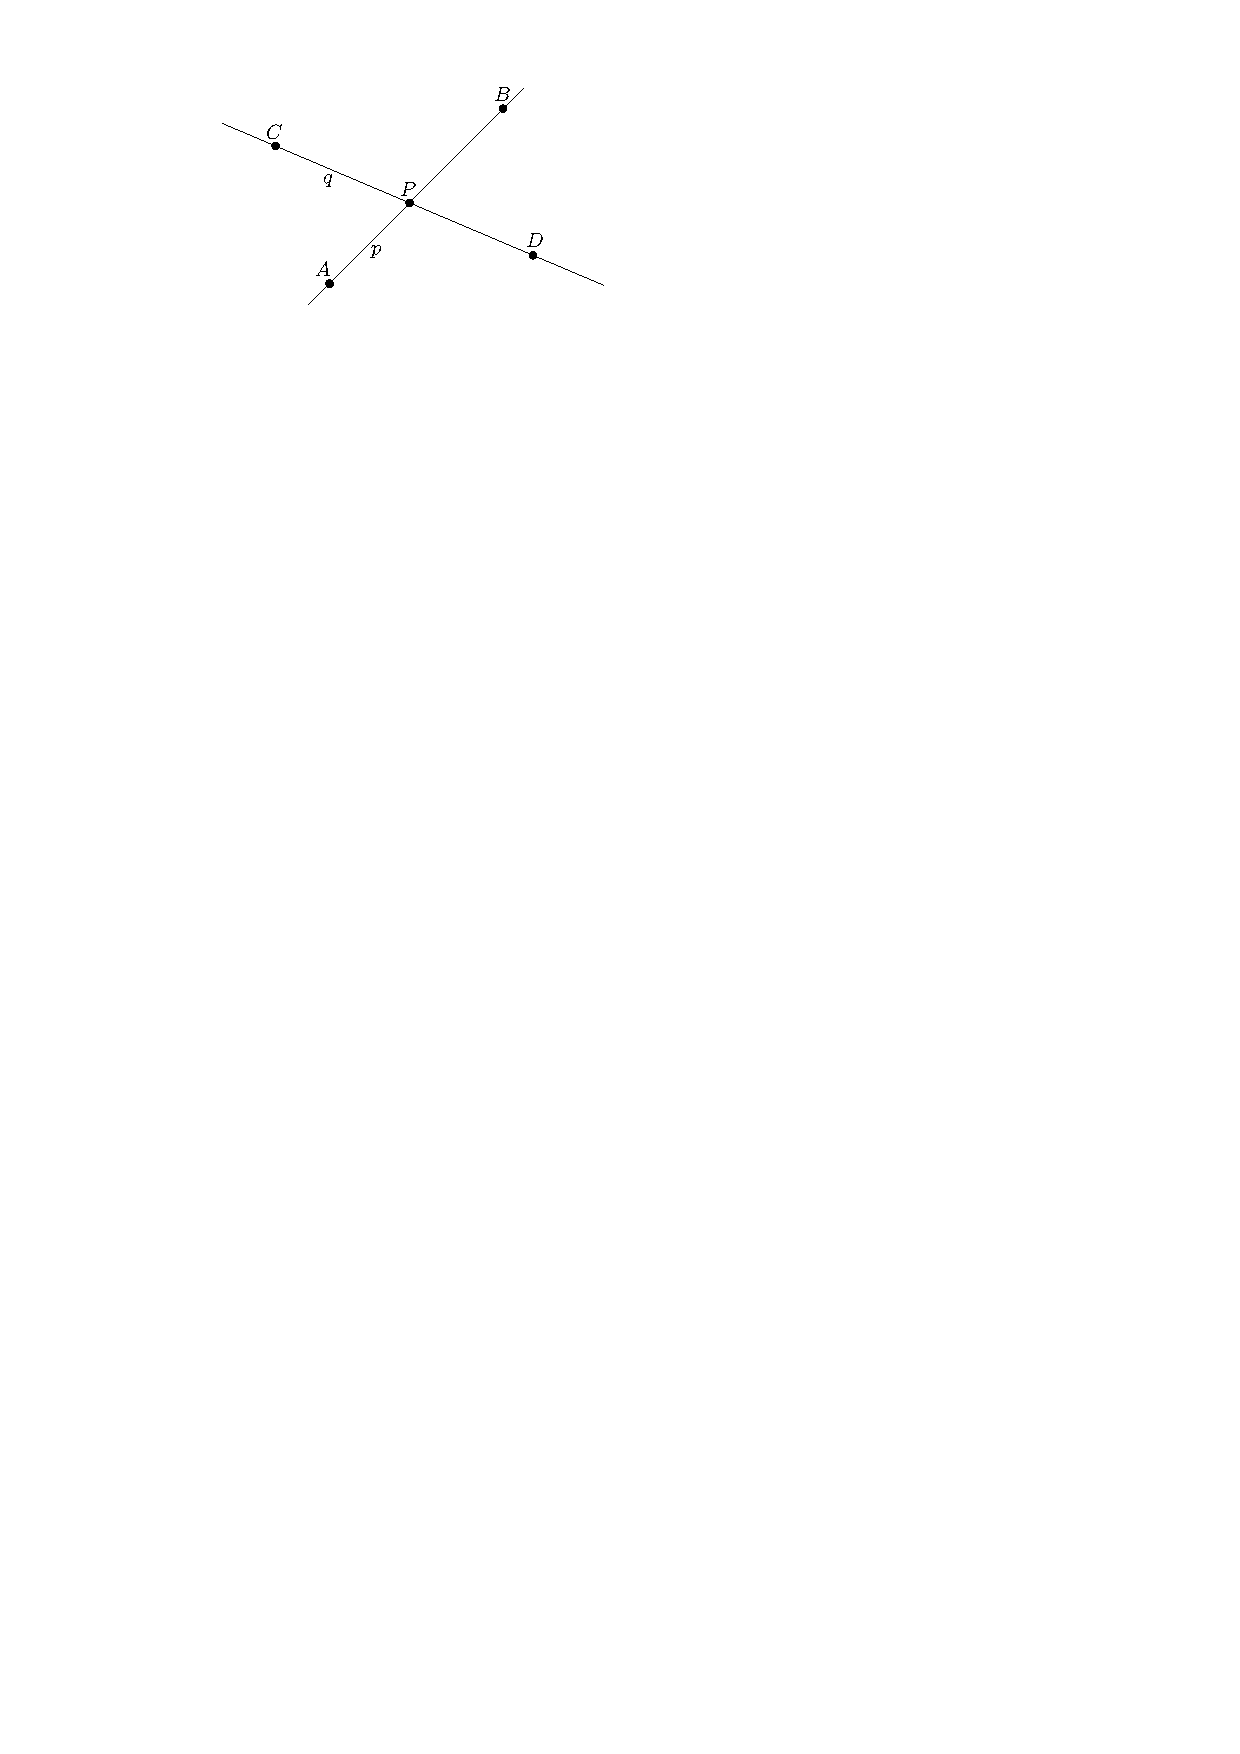
\includegraphics{../img/prusecik.pdf}
	\caption{Průsečík dvou přímek}
	\label{fig:prusecik}
\end{figure}

Průsečík musí ležet na obou přímkách a proto musí splňovat jejich obecné rovnice
$ax+by+c=0$.  Vyjádřeme si nyní obecné rovnice obou přímek. To můžeme
nejjednodušeji udělat pomocí normálových vektorů přímek. Mějme směrové vektory
přímek $p$: $u = (x_2-x_1,y_2-y_1)$ a $q$: $v=(x_4-x_3,y_4-y_3)$ pak normálové
vektory získáme jako $m = (-u_y,u_x)$ a $n = (-v_y,v_x)$. Obecná rovnice přímky
$p$ pak bude $m_xx+m_yy=c$ a přímky $q$ bude $n_xx+n_yy=d$. Koeficienty $c$ a
$d$ získáme dosazením bodů $A$ a $C$ do rovnic: $c = m_xx_1+m_yy_1$,
$d=n_xx_3+n_yy_3$. Pro průsečík musí platit obě rovnice, tedy 
\begin{eqnarray*}
m_xx+m_yy &=& m_xx_1+m_yy_1\\
n_xx+n_yy &=& n_xx_3+n_yy_3
\end{eqnarray*}
Tuto soustavu dvou rovnic o~dvou neznámých můžeme řešit například pomocí
determinantů Cramerovým pravidlem:

$$x = \frac{
	\begin{vmatrix}
		c & m_y \\
		d & n_y
	\end{vmatrix}
}
{
	\begin{vmatrix} 
		m_x & m_y \\
		n_x & n_y 
	\end{vmatrix}
}\,\!,\qquad
y = \frac{
	\begin{vmatrix}
		m_x & c \\
		n_x & d
	\end{vmatrix}
}
{
	\begin{vmatrix} 
		m_x & m_y \\
		n_x & n_y 
	\end{vmatrix}
}
$$

Pokud vzorec roznásobíme, získáme pro $x$-ovou souřadnici zlomek:
$$
x=\frac{(x_1 y_2-y_1 x_2)(x_3-x_4)-(x_1-x_2)(x_3 y_4-y_3 x_4)}
{(x_1-x_2)(y_3-y_4)-(y_1-y_2)(x_3-x_4)}$$
Tímto výrazem pak dokážeme jednoduše spočítat průsečík dvou přímek, pokud známe
souřadnice dvou bodů na každé z~nich.

\section{Reprezentace čísel}
V~průběhu dalšího zpracování budeme potřebovat počítat průsečíky úseček daných
uzly. Protože průsečíky úseček nebudou mít celočíselné souřadnice, je potřeba
rozmyslet, jakým způsobem je reprezentovat.

{\tuc Čísla s~plovoucí desetinnou čárkou} se pro tyto účely nehodí, protože
nejsou přesná. Při výpočtech s~nimi vznikají zaokrouhlovací chyby, které mohou
zapříčinit špatné pořadí blízkých průsečíků v~uspořádání. Potřebujeme proto
přesnou reprezentaci.

{\tuc Zlomky} jsou pro reprezentaci desetinných čísel vhodnější. Dokážeme pomocí
nich přesně reprezentovat desetinná čísla. Zlomky můžeme vždy
upravit tak, aby jejich jmenovatel byl kladný.  Takové zlomky můžeme porovnávat
podle pravidla $\frac{a}{b} < \frac{c}{d} \Leftrightarrow a\cdot d < c\cdot b $. 
Pokud se nám ale stane, že porovnáváme dva zlomky, které mají vysoký čitatel i
jmenovatel, nemusí nám 64 bitů přesnosti stačit.

Předpokládejme, že máme město velikosti Prahy, což je přibližně $20 \times
30$\,km s~přesností na 10\,cm. O~úsečkách víme, že žádná nebude delší než 300
metrů, tudíž rozdíl jejich souřadnic nebude větší než 3\,000. Pokud budeme
maximalizovat jmenovatele, ze vzorce pro výpočet průsečíku vychází, že můžeme
dosáhnout nejvýše 9 milionů, protože jde o~součin dvou rozdílů souřadnic a každý
bude nejvýše 3\,000.

Tato situace opravdu může nastat, například pro vodorovnou a svislou úsečku
o~délce 300\,m, dotýkající se v~krajním bodě, tzn. $A=(3\,000,0),B=(0,0)$,
$C=(0,3\,000),D=(0,0)$. Tyto dvě mají průsečík, tudíž se nám mohou při počítání
vyskytnout. Pokud nyní vezmeme téměř totožnou situaci, ale úsečky budou posunuty
směrem k~maximu $x$-ové osy, pak bude $x$-ová souřadnice reprezentovat číslo
30\,km při přesnosti 10\,cm ve zlomku se jmenovatelem 9 milionů. Bude to tedy
číslo $30\cdot1\,000\cdot10\cdot9\cdot10^6=27 \cdot 10^{11}$. Na reprezentaci tohoto
čísla budeme potřebovat $\log_2 (27\cdot 10^{11}) \doteq 42$ bitů. Pokud tento
zlomek budeme chtít porovnat s~jiným zlomkem s~maximálním jmenovatelem, budeme
potřebovat $42 + \log_2 (9\cdot 10^{6}) \doteq 65$ bitů, na což nám 64bitová proměnná
nebude stačit.

{\tuc Smíšená čísla} nemají ani jednu z~předchozích nevýhod. Jsou to čísla,
která mají tvar $a+\frac{b}{c}$, kde $\frac{b}{c}<1$. Číslo $a$ nazvěme
základem, $b$ čitatelem a $c$ jmenovatelem. U~smíšených čísel je stejně jako
u~zlomků zachována přesnost, ale můžeme je porovnávat bez rizika přetečení.
Pokud se čísla liší v~základu, pak přeteční nehrozí, protože základy se
porovnávají přímo. Pokud mají dvě smíšená čísla stejné základy, pak porovnáme
jejich zlomky. To ale na rozdíl od přímého porovnávání zlomků není problém,
protože jmenovatel je opět nejvýše 24bitový a protože čitatel je nejvýše tak
velký jako jmenovatel, jejich vynásobením vznikne nejvýše 48bitové číslo.
Protože proměnné máme 64bitové, nikde k~přetečení nedojde.

Smíšená čísla jsou implementována jako struktury se členy \verb|base| pro
základ, \verb|numer| pro čitatele a \verb|denom| pro jmenovatele. Všechny
položky jsou 64bitová celá čísla a jmenovatel nesmí být záporný. Pro práci se
smíšenými čísly jsou definovány pomocné funkce v~souboru \verb|mixnum.h|.

\section{Spojky mezi cestami}
\subsection{Příprava dat}
Spojky budeme vytvářet mezi cestami, po kterých budeme posléze vyhledávat.
Nejprve si proto všechny cesty ve funkci \verb|makeGraph| projdeme a roztřídíme
do dvou polí. 

Pole \verb|wayGraph| obsahuje pro každý uzel pole všech jeho sousedů po cestách,
po kterých se bude vyhledávat. Pole \verb|barGraph| obsahuje ty dvojice indexů
uzlů, které spolu sousedí na některé cestě označené jako překážka. Obě pole
reprezentují graf, první pomocí seznamu sousedů, druhé pomocí seznamu hran.
Každé pole budeme využívat jiným způsobem, a proto se nám hodí různá
reprezentace.

Jako druhý krok nalezneme všechny kandidáty na spojky. Zde využijeme mřížky.
Protože spojky chceme dlouhé nejvíce 20 metrů a mřížka má čtverce o~hraně také
20 metrů, stačí nám při hledání možných spojek pro daný bod se podívat pouze na
body ve čtverci, kde sám leží, v~sousedních čtvercích napravo od něj (nahoře,
uprostřed a dole) a ve čtverci pod ním. Protože jsou spojky kratší než 20\,m,
nemohou dále než do sousedního čtverce dosáhnout a protože procházíme postupně
všechny čtverce, možné spojky doleva a nahoru již známe ze zpracování
předchozích čtverců. 

Jednotlivé počáteční a koncové body spojek získáme ze všech bodů v~daném čtverci
vytříděním těch, které mají nějaké sousedy v~poli \verb|wayGraph|. Nepřidáváme
ale všechny spojky, protože pak existovalo např. u~kruhových cest v~parcích
mnoho spojek, které nepřinášely výrazné zlepšení. Zvolili jsme proto náhodný
výběr, při němž pro každý bod vybereme z~každého čtverce mřížky jen několik
kandidátů. Zkoumali jsme vliv počtu kandidátů na délku trasy a jako optitmum se
ukázalo zvolit dva body jako kandidáty z~každého čtverce mřížky. Při větším
množství bodů se výslledky zlepšovaly přibližně o~procento, ale velikost
výstupního souboru rostla přibližně o~šest procent.

%TODO: obrázek

\subsection{Datové struktury}
Když máme připravené kandidáty na spojky a seznam všech překážek, můžeme
přistoupit k~zametání roviny. Zametání roviny probíhá ve funkci
\verb|findDirectWays|. Nejprve popíšeme používané struktury a proměnné.

Struktura \verb|line_t| reprezentuje úsečku v~rovině. Při vytváření se jí
nastavují tyto atributy:
\begin{itemize}
	\item \verb|startlon| a \verb|startlat| udávají souřadnice začátku
	úsečky. Začátek úsečky má vždy nejvýš tak velkou souřadnici $x$, jako
	konec.
	\item \verb|endlon| a \verb|endlat| udávají souřadnice konce úsečky.
	Souřadnice začátků a konců jsou vždy celočíselné, proto je
	reprezentujeme 64bitovými celými čísly.
	\item \verb|startid| a \verb|endid| udávají identifikátor začátku a
	konce úsečky v~OSM.
	\item \verb|isBar| říká, jestli je daná úsečka překážkou.
\end{itemize}
V~průběhu zametání roviny jsou úsečkám nastavovány následující atributy:
\begin{itemize}
	\item \verb|broken| říká, jestli má průsečík s~jinou úsečkou a alespoň
	jedna z~nich je překážka.
	\item \verb|started| udává, že byla zařazena do průřezu.
	\item \verb|ended| udává, že byla v~průžezu a již skončila.
\end{itemize}

Globální pole \verb|lines| s~prvky typu \verb|line_t| obsahuje všechny kandidáty
na spojky, globální pole \verb|bars| s~prvky typu \verb|line_t| obsahuje všechny
překážky. 

Pro zametání budeme také potřebovat haldu, ze které budeme vybírat nejbližší
událost. V~našem případě používáme haldy dvě, první (\verb|seQueue|), kterou na
začátku naplníme událostmi začátek a konec úsečky, a druhou (\verb|intQueue|),
kterou budeme průběžně plnit průsečíkovými událostmi. V~každém průběhu hlavního
cyklu pak vybereme tu událost, která nastane dříve. Samotné haldy jsou pak
reprezentovány v~poli pomocí binárních hald z~LibUCW. 

Haldy obsahují struktury typu \verb|event_t| respektive \verb|int_event_t| pro
počáteční a koncové respektive průsečíkové události. Struktury mají následující
prvky:
\begin{itemize}
	\item \verb|lon| a \verb|lat| udávají souřadnice události. V~případě
	začátků a konců se jedná o~64bitová celá čísla, v~případě průsečíků se
	jedná o~čísla smíšená. 
	\item \verb|dlon| a \verb|dlat| udávají směrnici úsečky, které se
	událost týká. V~případě průsečíků se jedná o~tu, která by byla
	zpracována dříve.
	\item \verb|lineIdx| je index úsečky, které se událost týká
	\item \verb|line2Idx| se vyskytuje pouze u~průsečíků a jde o~index druhé
	úsečky, které se událost týká.
\end{itemize}


\subsection{Reprezentace průřezu}
Také budeme potřebovat vyhledávací strom, ve kterém si budeme pamatovat aktuální
pořadí úseček v~průřezu. Pro jeho reprezentaci jsme zvolili červeno-černé stromy
z~LibUCW. V~jeho vrcholech jsou uloženy jednotlivé úsečky, které jsou aktuální
pro daný průřez. Protože se ale úsečky mohou křížit, použili jsme několik
vlastních rozšíření. 

Museli jsme si napsat vlastní {\tuc porovnávací funkci}. Zametáme podle $x$-ové
souřadnice tudíž ve stromě potřebujeme mít úsečky seřazené podle $y$-ové
souřadnice v~daném bodě. Ta se ale s~kažým posunutím zametací přímky mění,
proto ve stromě najdeme pouze indexy do pole \verb|lines| na jednotlivé úsečky.
Porovnávací funkce dostane tyto indexy, z~globální proměnné \verb|lon| zjistí,
jaká je aktuální $x$-ová souřadnice zametací přímky, a vypočítá $y$-ovou
souřadnici porovnávaných úseček v~daném bodě. Pokud se $y$-ové souřadnice liší,
pak vrátí výsledek, pokud jsou shodné, porovnávají se podle úhlu. 

K~tomuto je zapotřebí globální proměnná \verb|anglesign|, která říká, s~jakým
znaménkem se má úhel brát. Pokud totiž srovnáváme úsečky při přidávání, zajímá
nás, v~jakém úhlu pokračují dále, naopak při odebírání nás zajímá, pod jakým
úhlem přicházejí. Seřazení je v~tomto případě přesně opačné. Úsečka, která
mířila nejvíce k~severu, tudíž byla na začátku poslední z~daného bodu, bude na
konci přicházet z~jihu, tudíž bude mezi prvními. Úhly úseček nepotřebujeme
počítat, stačí nám porovnat jejich směrnice, což jsou zlomky, a to umíme rychle
a beze ztráty přesnosti.

Ve stromě dále musíme umět prohodit dva sousední vrcholy při průsečíku jim
odpovídajících úseček. Protože si ve vrcholech pamatujeme pouze indexy do pole
úseček, stačí při překřížení tyto indexy prohodit. Struktura stromu i korektnost
uspořádání tím zůstanou zachovány.

Stromy v~LibUCW umí i mazání vrcholu podle pointeru na něj, což se nám hodí při
událostech konec úsečky, protože ji nemusíme hledat, ale stačí si při vytváření
úsečky uložit pointer na vrchol stromu do pole \verb|lineNodes| a při křížení
úseček prohodit patřičné ukazatele. Při mazání se pak jen podíváme podle indexu
úsečky do správného místa v~poli a patřičný vrchol smažeme. Je to výhodou i
v~situaci, kdy nastal při zametání nějaký problém a neproběhla nějaká událost
křížení, a tudíž bychom standardní cestou vrchol nenašli.

Při vkládání nového vrcholu do stromu také potřebujeme zjistit sousedy nově
vloženého vrcholu, abychom přidali případné události křížení. Tuto funkci stromy
v~LibUCW již také obsahují, tudíž nám stačí ji jen využít. Sousedy rovněž
hledáme při křížení, protože překřížením úseček se sousedství změnilo.


\subsection{Zametání}
Události procházíme seřazené nejprve podle délky, pak podle šířky. Pokud jsou
dvě události na stejném místě, nejprve se zpracují události konce úsečky, poté
průsečíky a nakonec události začátku úsečky. Pokud nastane více událostí téhož
typu na stejném místě, zpracovávají se podle úhlu úseček, viz rozbor pořadí ve stromě. 

Dokud máme v~haldě nějaké události, vybereme vždy tu nejbližší a zpracujeme ji.
Pokud se jedná o~začátek úsečky, zkontrolujeme, jestli ve stromě již není, či
zda v~něm není nějaká, se kterou by byla nerozlišitelná. Protože dvě úsečky,
které leží přesně přes sebe, se v~korektních datech nemohou vyskytovat, tak tu 
úsečku, která přijde ke
zpracování jako druhá, ignorujeme. Úsečku následně vložíme do průřezového stromu
a zkontrolujeme sousední úsečky, zda se s~nově přidanou nekříží. Pokud ano, tak
přidáme příslušné průsečíkové události do průsečíkové haldy.

Jedná-li se o~konec úsečky, zkontrolujeme, zda úsečka začala (byla přidána do
stromu). Pokud ne, skončíme. Následně zjistíme, zda odstraněním této úsečky se
její sousedé neprotnou, případně přidáme průsečíkovou událost. Nakonec úsečku
smažeme z~průřezového stromu.

Pokud se jedná o~průsečík, nejprve zkontrolujeme, jestli jsme danou událost již
nezpracovali. Pokud se totiž dvě úsečky protínají a během toho, co se k~sobě
přibližují se mezi nimi objeví další úsečka, vznikne průsečíková událost těchto
dvou krajních přímek poprvé při přidání pozdější z~nich a podruhé při konci
vnitřní úsečky, přitom se stále jedná o~stejný průsečík. Protože tyto dvě
průsečíkové události se seřadí hned za sebe a protože se každé dvě úsečky
protnou nejvýše jednou, stačí nám si pamatovat poslední událost a pokud je nová
průsečíková událost se stejnými úsečkami, můžeme ji zahodit.

Dále zkontrolujeme, jestli některá z~úseček již neskončila. Pokud se dvě úsečky
potkávají v~koncovém bodě, pak je zbytečné řešit jejich průsečík. Proto nejprve
vyřešíme konce úseček a pokud máme řešit průsečík s~již skončenou úsečkou,
můžeme ho ignorovat. Následně zjistíme, která z~úseček je nyní horní a která
dolní, a prohodíme odkazy na vrcholy stromu v~poli \verb|lineNodes| a rovněž
prohodíme indexy úseček ve vrcholech stromu. Nakonec zjistíme, zda po prohození
nevznikly nové průsečíky, a případně přidáme průsečíkové události.

Když celý cyklus doběhne, přidáme funkcí \verb|addDirectToMap| do seznamu cest
nově vzniklé spojky a jsme hotovi.


\section{Zkratky přes průchozí prostranství}
Abychom mohli vytvářet zkratky přes průchozí prostranství, potřebujeme nejprve
zjistit, které všechny uzly se vyskytují v~tomto prostranství. Pro samotné
vytváření zkratek pak použijeme obdobný způsob jako při hledání spojek mezi
cestami. 

Nejprve vytvoříme pole všech průchozích prostranství.  K~tomuto účelu
slouží funkce \verb|findWalkAreas|. Procházíme postupně všechny cesty a u~každé
kontrolujeme, jestli se jedná o~průchozí prostranství. Pokud ano, pak vytvoříme
strukturu \verb|walk_area_t| obsahující data o~této ploše: Zjistíme, do jakého
podobélníku mřížky plocha zasahuje, a z~tohoto podobdélníku vybereme ty body,
které jsou uvnitř plochy. Body přidáme do pole \verb|nodeIdxs| a cesty do pole
\verb|ways|. Cesty potom rozdělíme na překážky, jejichž indexy uložíme do
atributu \verb|barIdxs| a vyhledávatelné cesty, které uložíme do atributu
\verb|wayIdxs|. Během rozdělování také odstraňujeme duplicitní cesty. 

Jako další krok připravíme kandidáty na zkratky. Použijeme k~tomu funkci
\verb|makeAreaCandidates|. Procházíme postupně dvojice bodů v~dané ploše a
hledáme bližší než 300\,m, které nejsou na společné cestě. Neuvažujeme ovšem
všechny dvojice, ale vybíráme pro každý uzel náhodně z~ostatních uzlů, protože
při uvažování všech dvojic vznikalo mnoho cest v~podobných místech podobným
směrem. Nalezené dvojice následně přidáme do seznamu kandidátů. Experimentálně
jsme zkoumali vliv průměrného počtu sousedů pro jeden vrchol na délku nalezených
cest přes pražskou Stromovku a Letnou. Jako optimální se ukázalo vybírat pro
každý vrchol průměrně dva sousedy. K~dalšímu výrazném zlepšení totiž došlo až
pro pět sousedů, což ale při zlepšení o~přibližně 10 procent vedlo ke zvýšení
velikosti grafu o~20 procent, což nám již  přišlo nevýhodné.

Vytvoříme také seznam překážek funkcí \verb|makeAreaBarGraph|. Nejprve přidáme
všechny překážky ze seznamu \verb|barIdxs|, poté přidáme všechny cesty
z~\verb|wayIdxs| a nakonec přidáme obvod plochy. Cesty přidáváme proto, aby
nevnikalo příliš mnoho zkratek, což by vedlo ke zvětšování vyhledávacího grafu.
Takto vzniknou pouz zkratky přes volná prostranství a nebudou křížit cesty.

Když máme kandidáty na zkratky i seznam překážek, můžeme použít již popsané funkce
\verb|findDirectWays| a \verb|addDirectToMap| k~odstranění kandidátů
kolidujících
s~překážkami a cestami a k~přidání výsledných zkratek do mapy. Postup od přípravy
kandidátů až po jejich přidání do mapy zopakujeme pro každou průchozí plochu.

\section{Vytvoření vyhledávacího grafu}
Když již máme všechna data připravená, vytvoříme vyhledávací graf. Nejprve do
něj přidáme všechny vrcholy a hrany. Následně graf projdeme do hloubky a
vybereme tu komponentu, která je největší. Poté v~grafu necháme jen vrcholy a
hrany, které do této komponenty patří, a graf uložíme do souboru
\verb|praha-graph.pbf|. 
